
\section{觀念與公式}

\subsection{直線方程式}
直線是平面上最簡單的幾何圖形,常用以下形式表示:
\begin{itemize}
    \item \textbf{斜截式}:$y = mx + b$,其中$m$為斜率,$b$為$y$軸截距。
    \item \textbf{一般式}:$ax + by + c = 0$,適用於所有直線(包括垂直線)。
    \item \textbf{兩點式}:給定兩點$(x_1, y_1)$和$(x_2, y_2)$,方程式為:
    \[
    y - y_1 = \frac{y_2 - y_1}{x_2 - x_1} (x - x_1)
    \]
    \item \textbf{參數式}:$x = x_0 + at$,$y = y_0 + bt$,其中$(a, b)$為方向向量。
\end{itemize}
\textbf{性質}:
\begin{itemize}
    \item 斜率$m = \tan\theta$,$\theta$為與$x$軸夾角。
    \item 兩直線平行若$m_1 = m_2$,垂直若$m_1 \cdot m_2 = -1$。
    \item 點到直線距離:點$(x_0, y_0)$到$ax + by + c = 0$的距離為:
    \[
    d = \frac{|ax_0 + by_0 + c|}{\sqrt{a^2 + b^2}}
    \]
\end{itemize}
\textbf{應用}:描述軌跡、計算距離。\\
\textbf{大學技巧}:用向量法求距離,設直線法向量為$(a, b)$,點到直線的投影更快。

\subsection{圓方程式}
圓是以中心點為基準,所有點到中心的距離相等的圖形:
\begin{itemize}
    \item \textbf{標準式}:$(x - h)^2 + (y - k)^2 = r^2$,中心$(h, k)$,半徑$r$。
    \item \textbf{一般式}:$x^2 + y^2 + Dx + Ey + F = 0$,轉換為標準式:
    \[
    x^2 + Dx + \left(\frac{D}{2}\right)^2 + y^2 + Ey + \left(\frac{E}{2}\right)^2 = \frac{D^2 + E^2 - 4F}{4}
    \]
    中心$\left(-\frac{D}{2}, -\frac{E}{2}\right)$,半徑$r = \sqrt{\frac{D^2 + E^2 - 4F}{4}}$(若$D^2 + E^2 - 4F > 0$)。
\end{itemize}
\textbf{性質}:
\begin{itemize}
    \item 圓周上的點滿足方程式。
    \item 切線斜率:圓上點$(x_0, y_0)$的切線斜率為$\frac{h - x_0}{y_0 - k}$。
\end{itemize}
\textbf{應用}:軌跡問題、幾何優化。\\
\textbf{大學技巧}:用參數式$x = h + r\cos\theta$,$y = k + r\sin\theta$快速生成圓上點。

\subsection{直線與圓的關係}
直線$ax + by + c = 0$與圓$(x - h)^2 + (y - k)^2 = r^2$的位置關係:
\begin{itemize}
    \item \textbf{距離判別}:中心$(h, k)$到直線距離$d = \frac{|ah + bk + c|}{\sqrt{a^2 + b^2}}$:
    \[
    \begin{cases}
    d > r & \text{相離(無交點)} \\
    d = r & \text{相切(1交點)} \\
    d < r & \text{相交(2交點)}
    \end{cases}
    \]
    \item \textbf{交點計算}:將直線代入圓方程式,解二次方程:
    \[
    \Delta = r^2(a^2 + b^2) - (ah + bk + c)^2
    \]
    $\Delta > 0$(2交點),$\Delta = 0$(1交點),$\Delta < 0$(無交點)。
\end{itemize}
\textbf{應用}:判斷位置、求切線。\\
\textbf{大學技巧}:用幾何性質(如垂徑定理)或向量內積快速判斷關係。

\section{例題解析}

\subsection{例題1:直線方程式(計算題)}
求過點$(2, 3)$且與直線$3x - 4y + 5 = 0$平行的直線方程式。\\
\textbf{解}:原直線斜率$m = \frac{3}{4}$,平行直線斜率相同。用點斜式:
\[
y - 3 = \frac{3}{4} (x - 2) \implies 4y - 12 = 3x - 6 \implies 3x - 4y + 6 = 0
\]
\textbf{大學技巧}:法向量$(3, -4)$,新直線為$3x - 4y + c = 0$,代入$(2, 3)$得$c = 6$。

\subsection{例題2:圓方程式(計算題)}
將$x^2 + y^2 - 4x + 6y - 12 = 0$化為標準式,求圓心與半徑。\\
\textbf{解}:配方:
\[
x^2 - 4x + 4 + y^2 + 6y + 9 = 12 + 4 + 9
\]
\[
(x - 2)^2 + (y + 3)^2 = 25
\]
圓心$(2, -3)$,半徑$5$。\\
\textbf{大學技巧}:直接用公式,中心$\left(2, -3\right)$,$r = \sqrt{4 + 9 + 12} = 5$。

\subsection{例題3:直線與圓關係(應用題)}
判斷直線$y = x - 1$與圓$x^2 + y^2 = 4$的關係。\\
\textbf{解}:代入$y = x - 1$:
\[
x^2 + (x - 1)^2 = 4 \implies x^2 + x^2 - 2x + 1 = 4 \implies 2x^2 - 2x - 3 = 0
\]
判別式:
\[
\Delta = (-2)^2 - 4 \cdot 2 \cdot (-3) = 4 + 24 = 28 > 0
\]
有2交點,相交。\\
\textbf{大學技巧}:中心$(0, 0)$到直線距離$d = \frac{|0 - 0 - 1|}{\sqrt{1^2 + 1^2}} = \frac{1}{\sqrt{2}} < 2$,相交。

\subsection{例題4:幾何技巧(觀念題)}
求點$(3, 4)$到直線$2x + y - 5 = 0$的距離。\\
\textbf{解}:公式:
\[
d = \frac{|2 \cdot 3 + 1 \cdot 4 - 5|}{\sqrt{2^2 + 1^2}} = \frac{|6 + 4 - 5|}{\sqrt{5}} = \frac{5}{\sqrt{5}} = \sqrt{5}
\]
\textbf{大學技巧}:設垂足$(x, y)$,直線斜率$-\frac{2}{1}$,垂線斜率$\frac{1}{2}$,聯立解得交點$(2, 1)$,距離$\sqrt{(3-2)^2 + (4-1)^2} = \sqrt{5}$。

\section{圖形展示}
直線$y = x - 1$與圓$x^2 + y^2 = 4$:
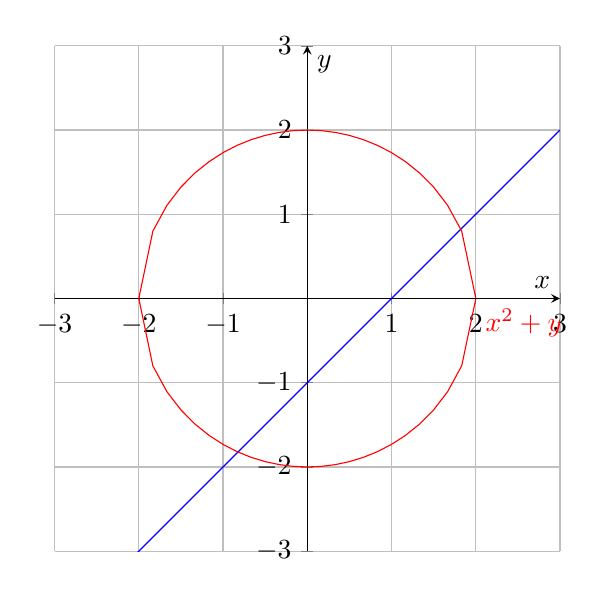
\begin{tikzpicture}
    \begin{axis}[
        axis lines=middle,
        xlabel=$x$,
        ylabel=$y$,
        xmin=-3, xmax=3,
        ymin=-3, ymax=3,
        grid=both,
        width=8cm, height=8cm
    ]
    \addplot[domain=-3:3, blue] {x-1} node[above right] {$y = x - 1$};
    \addplot[domain=-2:2, red] {sqrt(4-x^2)};
    \addplot[domain=-2:2, red] {-sqrt(4-x^2)} node[below right] {$x^2 + y^2 = 4$};
    \end{axis}
\end{tikzpicture}

\section{題庫}
\begin{enumerate}[label=\arabic*.]
    % 計算題 (10)
    \item 求過$(1, -2)$且斜率為$3$的直線方程式。
    \item 將$x^2 + y^2 + 2x - 4y - 4 = 0$化為標準式。
    \item 求直線$2x - 3y + 6 = 0$的斜率與截距。
    \item 求過$(0, 0)$與$(3, 4)$的直線方程式。
    \item 求圓$(x - 1)^2 + (y + 2)^2 = 9$的中心與半徑。
    \item 求點$(2, 1)$到直線$x + y - 3 = 0$的距離。
    \item 判斷直線$y = 2x$與圓$x^2 + y^2 = 1$的關係。
    \item 求過$(1, 1)$且與$x - 2y + 3 = 0$垂直的直線方程式。
    \item 求直線$x = 2$與圓$x^2 + y^2 - 4x = 0$的交點。
    \item 求點$(0, 5)$到直線$3x - 4y + 10 = 0$的距離。
    % 應用題 (10)
    \item 一點沿直線$y = x + 1$移動,求其到$(2, 0)$的最短距離。
    \item 求圓心在$(0, 0)$,過點$(3, 4)$的圓方程式。
    \item 若直線與圓$x^2 + y^2 = 5$相切,求直線斜率(過$(2, 3)$)。
    \item 求點$(1, 1)$到直線$y = -x + 2$的垂足坐標。
    \item 一圓過$(0, 0)$與$(2, 2)$,中心在$x$軸上,求方程式。
    \item 求直線$y = x$與圓$x^2 + y^2 - 2x - 2y + 1 = 0$的交點。
    \item 若直線$kx + y - 2 = 0$與圓$x^2 + y^2 = 2$相交,求$k$範圍。
    \item 求過$(3, 0)$且與圓$x^2 + y^2 = 4$相切的直線方程式。
    \item 一點到直線$2x - y + 1 = 0$的距離為$\sqrt{5}$,求坐標。
    \item 求圓心$(1, 1)$,半徑$2$的圓上斜率為$1$的點。
    % 觀念題 (10)
    \item 證明兩直線垂直時,斜率乘積為$-1$。
    \item 若圓一般式$D^2 + E^2 - 4F < 0$,圖形為何?
    \item 直線與圓相離時,判別式$\Delta$如何?
    \item 說明點到直線距離公式的幾何意義。
    \item 若直線過圓心,交點數為何?
    \item 證明圓的切線垂直於半徑。
    \item 兩直線平行時,法向量有何關係?
    \item 圓心到直線距離等於半徑時,關係為何?
    \item 說明如何用參數式表示直線。
    \item 證明直線$ax + by + c = 0$的法向量為$(a, b)$。
    % 進階題 (10)
    \item 求直線$y = x - 2$與圓$x^2 + y^2 - 4x = 0$的交點。
    \item 若直線與圓$x^2 + y^2 - 2x + 2y - 1 = 0$相切,求直線方程式(過$(0, 0)$)。
    \item 求點$(2, 3)$到直線$x - y + 1 = 0$的垂線方程式。
    \item 求圓$x^2 + y^2 = 1$上距離直線$y = x$最遠的點。
    \item 若直線$3x + 4y + k = 0$與圓$x^2 + y^2 = 5$相交,求$k$範圍。
    \item 求過$(1, 0)$且與圓$x^2 + y^2 - 2x = 0$相切的直線。
    \item 求直線$y = 2x - 1$與圓$x^2 + y^2 - 2y = 0$的弦長。
    \item 若圓心$(0, 0)$,過$(1, 1)$與$(2, 2)$,求方程式。
    \item 求直線$x + y = 1$與圓$x^2 + y^2 - x - y = 0$的交點。
    \item 若直線與圓相切,證明切點到圓心距離等於半徑。
    % 挑戰題 (20)
    \item 求過$(0, 0)$且與圓$x^2 + y^2 - 4x + 2y = 0$相切的直線。
    \item 若直線$y = mx + 1$與圓$x^2 + y^2 = 4$相交,求$m$範圍。
    \item 求點$(3, 4)$到直線$2x + 3y - 6 = 0$的垂足與距離。
    \item 求圓$x^2 + y^2 = 2$與直線$y = x - 1$的交點弦長。
    \item 若直線$ax + by + 1 = 0$與圓$x^2 + y^2 = 1$相切,求$a, b$關係。
    \item 求過$(2, 2)$且與圓$x^2 + y^2 - 2x - 2y + 1 = 0$相交的直線範圍。
    \item 求直線$y = x$與圓$x^2 + y^2 - 4x + 2y = 0$的交點。
    \item 若圓過$(0, 0)$,中心$(a, b)$,半徑$\sqrt{2}$,求方程式範圍。
    \item 求點$(1, 2)$到直線$3x - y + 1 = 0$的垂線與交點。
    \item 若直線與圓$x^2 + y^2 - 2x = 0$相離,求過$(0, 1)$的直線範圍。
    \item 求圓$x^2 + y^2 = 5$上到直線$x + y = 1$距離最大的點。
    \item 若直線$y = kx$與圓$x^2 + y^2 - 4 = 0$相切,求$k$。
    \item 求過$(0, 0)$與$(1, 1)$且與圓$x^2 + y^2 = 1$相交的直線。
    \item 若直線$2x + y + k = 0$與圓$x^2 + y^2 = 2$相切,求$k$。
    \item 求圓$x^2 + y^2 - 2x - 2y + 1 = 0$與直線$x - y = 0$的弦長。
    \item 若直線過$(3, 0)$與圓$x^2 + y^2 = 4$相交,求斜率範圍。
    \item 求點$(0, 0)$到直線$x - 2y + 4 = 0$的垂足與距離。
    \item 若圓心$(1, 1)$,過$(0, 0)$與$(2, 2)$,求方程式。
    \item 求直線$y = 2x - 3$與圓$x^2 + y^2 - 2x = 0$的交點。
    \item 若直線與圓$x^2 + y^2 = 1$相交,求過$(2, 0)$的直線範圍。
\end{enumerate}

